\documentclass[border=5pt]{standalone}
\usepackage{tikz}
\usepackage{amsmath}
\usetikzlibrary{calc,intersections}
\begin{document}
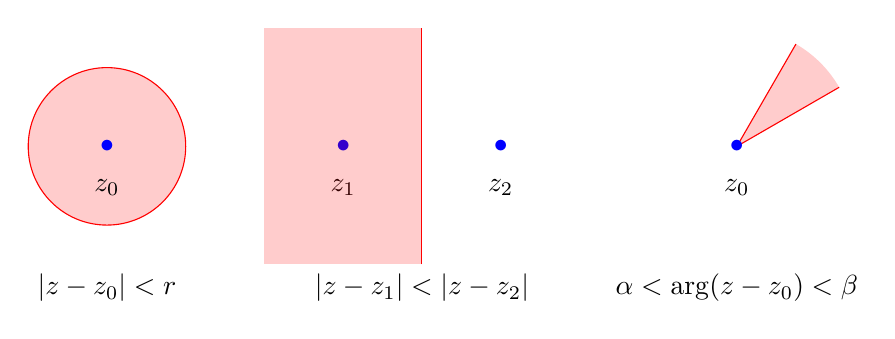
\begin{tikzpicture}[scale=1]
    % First diagram: |z-z0| < r
    \begin{scope}[xshift=-4cm]
        % Circle
        \draw[red] (0,0) circle (1);
        \fill[red, opacity=0.2] (0,0) circle (1);

        % Center
        \node[blue] at (0,0) {$\bullet$};
        \node[below] at (0,-0.3) {$z_0$};

        % Label
        \node[below] at (0,-1.5) {$|z-z_0| < r$};
    \end{scope}

    % Second diagram: |z-z1| < |z-z2|
    \begin{scope}[xshift=0cm]
        % Points
        \node[blue] at (-1,0) {$\bullet$};
        \node[below] at (-1,-0.3) {$z_1$};
        \node[blue] at (1,0) {$\bullet$};
        \node[below] at (1,-0.3) {$z_2$};

        % Perpendicular bisector
        \draw[red] (0,-1.5) -- (0,1.5);
        \fill[red, opacity=0.2] (-2,-1.5) rectangle (0,1.5);

        % Label
        \node[below] at (0,-1.5) {$|z-z_1| < |z-z_2|$};
    \end{scope}

    % Third diagram: α < arg(z) < β
    \begin{scope}[xshift=4cm]
        % Sector
        \draw[red] (0,0) -- ({1.5*cos(30)},{1.5*sin(30)});
        \draw[red] (0,0) -- ({1.5*cos(60)},{1.5*sin(60)});
        \fill[red, opacity=0.2] (0,0) -- ({1.5*cos(30)},{1.5*sin(30)}) arc (30:60:1.5) -- cycle;

        % Origin
        \node[blue] at (0,0) {$\bullet$};
        \node[below] at (0,-0.3) {$z_0$};

        % Label
        \node[below] at (0,-1.5) {$\alpha < \arg(z-z_0) < \beta$};
    \end{scope}
\end{tikzpicture}
\end{document}
